\documentclass{beamer}

\mode<presentation> 
{
    % The Beamer class comes with a number of default slide themes
    % which change the colors and layouts of slides. Below this is a list
    % of all the themes, uncomment each in turn to see what they look like.

    %\usetheme{default}
    %\usetheme{AnnArbor}
    %\usetheme{Antibes}
    %\usetheme{Bergen}
    %\usetheme{Berkeley}
    %\usetheme{Berlin}
    %\usetheme{Boadilla}
    %\usetheme{CambridgeUS}
    %\usetheme{Copenhagen}
    %\usetheme{Darmstadt}
    %\usetheme{Dresden}
    %\usetheme{Frankfurt}
    %\usetheme{Goettingen}
    %\usetheme{Hannover}
    %\usetheme{Ilmenau}
    %\usetheme{JuanLesPins}
    %\usetheme{Luebeck}
    \usetheme{Madrid}
    %\usetheme{Malmoe}
    %\usetheme{Marburg}
    %\usetheme{Montpellier}
    %\usetheme{PaloAlto}
    %\usetheme{Pittsburgh}
    %\usetheme{Rochester}
    %\usetheme{Singapore}
    %\usetheme{Szeged}
    %\usetheme{Warsaw}

    % As well as themes, the Beamer class has a number of color themes
    % for any slide theme. Uncomment each of these in turn to see how it
    % changes the colors of your current slide theme.

    %\usecolortheme{albatross}
    %\usecolortheme{beaver}
    %\usecolortheme{beetle}
    %\usecolortheme{crane}
    %\usecolortheme{dolphin}
    %\usecolortheme{dove}
    %\usecolortheme{fly}
    %\usecolortheme{lily}
    %\usecolortheme{orchid}
    %\usecolortheme{rose}
    %\usecolortheme{seagull}
    %\usecolortheme{seahorse}
    %\usecolortheme{whale}
    %\usecolortheme{wolverine}

%\setbeamertemplate{footline} % To remove the footer line in all slides uncomment this line
%\setbeamertemplate{footline}[page number] % To replace the footer line in all slides with a simple slide count uncomment this line

%\setbeamertemplate{navigation symbols}{} % To remove the navigation symbols from the bottom of all slides uncomment this line
}

\usepackage{graphicx} % Allows including images
\usepackage{booktabs} % Allows the use of \toprule, \midrule and \bottomrule in tables


\usepackage{beamerthemeshadow}
\usepackage{latexsym,amsbsy,amsopn,amstext,xcolor,multicol,amsmath}
\usepackage{amssymb,graphicx,wrapfig,fancybox}
\usepackage{pgf,pgfarrows,pgfnodes,pgfautomata,pgfheaps,pgfshade}
\usepackage{booktabs}
\usepackage{subfloat}
\usepackage{}
\graphicspath{{figures/}}

%----------------------------------------------------------------------------------------
%	TITLE PAGE
%----------------------------------------------------------------------------------------

\title[Group Report]{Group Report on Recent Work}

\author{Ma Hsuning}
\institute[NKU]
{
    Physics of NKU\\
    \medskip
    \textit{maxn@ihep.ac.cn}
}
\date{\today}

%----------------------------------------------------------------------------------------
\begin{document}
%----------------------------------------------------------------------------------------
\frame{\titlepage}
%----------------------------------------------------------------------------------------

\section{Optimization}
%----------------------------------------------------------------------------------------
\begin{frame}{Introduction}
We optimized the selection with ROOT scripts, with the max $S=\frac{N_S}{\sqrt{N_S+N_B}}$, where $S$ is the significance, $N_S$ is the number of signal events, and $N_B$ is the number of background events.\\
        \bigskip
And we used the signal MC to determine the number of signal events $N_S$, and the inclusive MC the number of background and signal events $N_S+N_B$, which we verified as a reasonable option.
\end{frame}
%----------------------------------------------------------------------------------------

\begin{frame}{Optimization}
We did topology analysis after we got the inclusive MC Results, and found the main background are:
    \begin{itemize}
    \item $\psi(3686) \rightarrow \pi^0 \pi^0 J/\psi$
    \item $\psi(3686)\rightarrow \gamma \chi_{cj}$
    \item $\psi(3686) \rightarrow \pi^+ \pi^- J/\psi$
    \end{itemize}
    \end{frame}
    %----------------------------------------------------------------------------------------
    \begin{frame}{Optimization Results}
    Using a ROOT scripts, we got the Optimization as below:
        \begin{itemize}
        \item $0<\chi_{4C}^2<25$;
        \item $0.125<m_{\pi^0}<0.138$;
        \item $0.45<E(\gamma_{E1})<0.53$;
        \item $|m_{recoil}(\pi^0 \pi^0)-M_{J/\psi}|<0.033$;
        \item $|m_{recoil}(\gamma)-M_{\chi_{c0}}|<0$;
        \item $|m_{recoil}(\gamma)-M_{\chi_{c1}}|<0.004$;
        \item $|m_{recoil}(\gamma)-M_{\chi_{c2}}|<0.002$;
        \item $|m_{recoil}(\pi^+ \pi^-)-M_{J/\psi}|<0.004$.
        \end{itemize}
        \end{frame}
        %----------------------------------------------------------------------------------------
        \section{Results after Optimization}
        \begin{frame}{Distribution of $m_{\eta_c}$}
        \begin{center}
        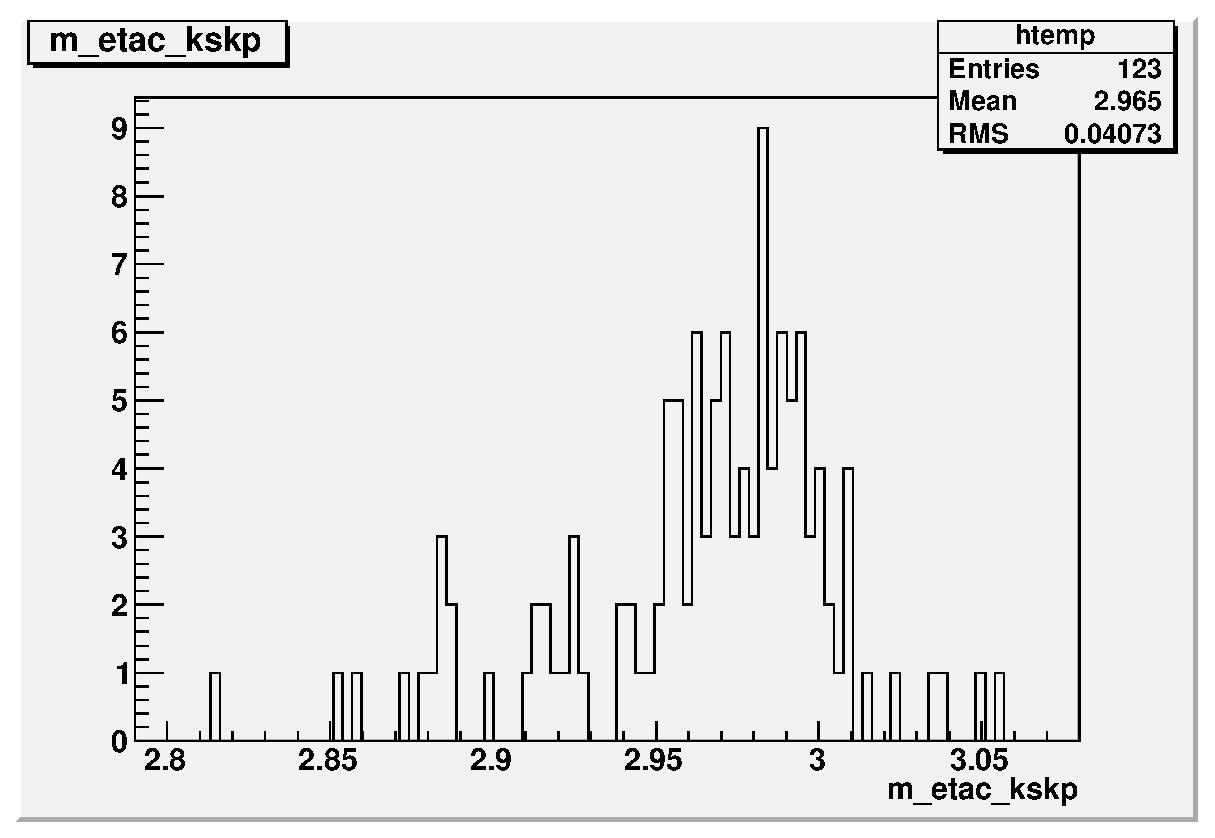
\includegraphics[width=0.9\textwidth,angle=0]{figures/Pi0hc_optimization_m_etac_kskp.eps}
        \end{center}
        \end{frame}
        %----------------------------------------------------------------------------------------
        \begin{frame}{Distribution of $m_{h_c}$}
        \begin{center}
        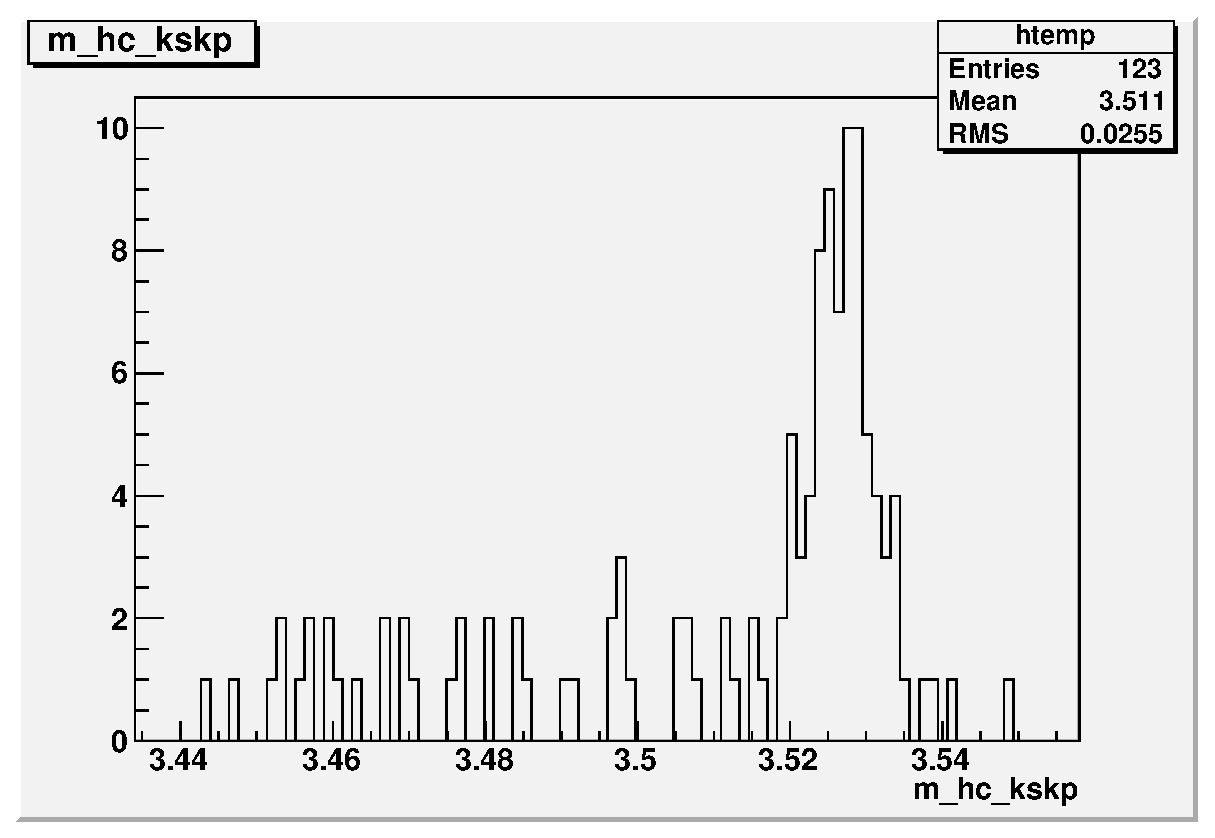
\includegraphics[width=0.9\textwidth,angle=0]{figures/Pi0hc_optimization_m_hc_kskp.eps}
        \end{center}
        \end{frame}
        %----------------------------------------------------------------------------------------
        \begin{frame}{Topology analysis}
        \begin{center}
        \vskip -2.0cm
        \includegraphics[width=0.8\textwidth,angle=270]{figures/notice.eps}
        \end{center}
        \end{frame}
        %----------------------------------------------------------------------------------------
        \section{Things to do}
        \begin{frame}
        \begin{itemize}
        \item Background analysis in 2-3 weeks
        \end{itemize}
        \end{frame}
        \end{document}
